
\chapter{Introduction}
\subitem
{
	\large{
	My name is Mohammed Elhossiny and we will talk about INTERNET OF THINGS in this book.
	\vspace{5mm} %5mm vertical space
	IOT: New Term, Means the new generation of the Internet, which allows understanding between devices interconnected with each (VoIP). These include hardware tools and sensors and sensors and the various tools of artificial intelligence and others. This definition goes beyond the traditional concept and which continues to persons with computers and smartphones through a single global network and through traditional Internet Protocol. What distinguishes the Internet of things it allows for a person to be free from the place, that any person can control the tools without having to be in a specific place to deal with a particular device.
	\vspace{5mm} %5mm vertical space
	We will discuss about the history, applications, interact technology, humanity with Internet of things and other interesting subjects. \hfill \break }

    \large{
    	    \vspace{5mm} %5mm vertical space
    hope to be useful to you \newline
    \textbf{ let's start...}
                }
            
	
}
\subitem{
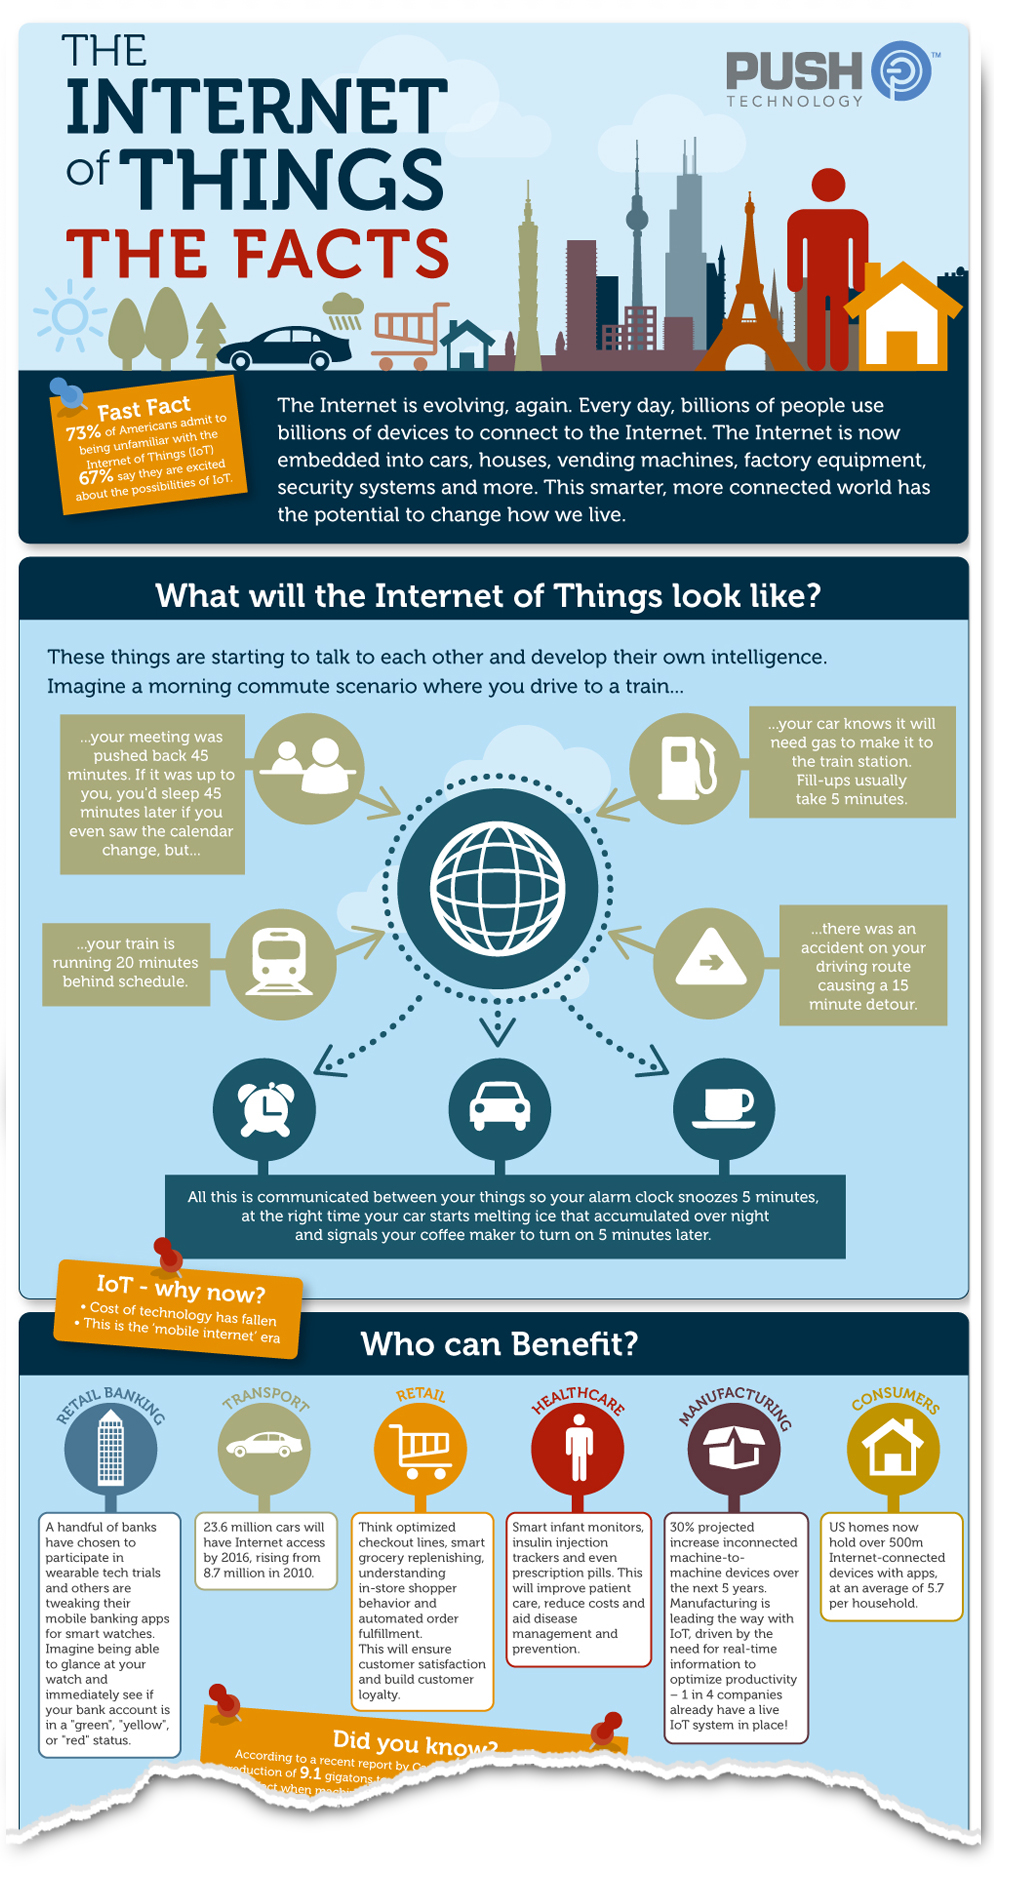
\includegraphics[width=\textwidth,height=\textheight,keepaspectratio]{IOT2.jpg}}